\section{Coarsening for Dynamics}
The realistic simulation of highly-dynamic elastic objects is important for a broad range of applications in computer graphics, engineering and computational fabrication.
However, whether simulating flipping toys, jumping robots, prosthetics or quickly moving creatures, performing such simulations in the presence of contact, impact and friction is both time consuming and inaccurate.
\emph{Coarsening} offers an exciting approach for efficient yet predictive FE modeling.
Analytical solutions for coarsening have been developed for linear material models (models where the stress varies linearly with strain)~\cite{Kharevych2009,Nesme2009,Torres:2016:HIC}.
Due to this linear assumption, we find them difficult to apply for the accurate modeling of the nonlinear materials required for 3D-printed objects.
Even though our proposed DDFEM overcomes the linear limitation of prior work, it does not account for dynamic effects, inertial properties, nor material damping characteristics.
We propose \textbf{Dynamics-Aware Coarsening} (DAC) and the \textbf{Boundary Balanced Impact} (BBI) model for the accurate simulation of dynamic, elastic objects undergoing both large scale deformation and frictional contact.
Our methods aim to balance efficiency and accuracy to enable design-for-fabrication optimization. They can be used for both fast, realistic animation and engineering analysis. 
\subsection{Dynamics-Aware Coarsening}
We couple numerical coarsening with material parameter acquisition.
Our DAC method computes \emph{numerical} stiffness parameters for the nonlinearly elastic, Neohookean material model, and damping parameters for the Rayleigh damping model to preserve the dynamic behavior of real-objects or high-resolution simulations.
Because the goal of DAC is to replicate the dynamic behavior of a high-resolution simulation, we focus on creating a coarse mesh which captures both the large-scale deformation modes, and the corresponding natural frequencies of the high-resolution mesh.
We do this in two stages. First, we produce a coarse hexahedral mesh that can replicate the large scale deformation modes of our high-resolution mesh.
Second, we compute material and damping parameters that yield matching fundamental frequencies for each mode shape on this coarse mesh.

DAC uses an iterative procedure to create the coarse mesh while maintaining mode shapes.
We initialize our mesh to a coarse hexahedral discretization of the starting geometry, $\mathbf{q}^0$, and then subdivide recursively until we reach a convergent mesh resolution.
We then solve the generalized mass-PCA system 
\begin{align}
\mathbf{K}(\mathbf{q}^0) \mathbf{q} = \lambda \mathbf{M}\mathbf{q}
\end{align}
for the dominant shape modes of the convergent system and then 
choose a maximally coarse mesh that matches the dominant four shape modes to tolerance. We use a relative geometric difference of $5\%$ (Hausdorff distance) as our tolerance threshold. Typically this is a short validation step as even the coarsest meshes generally satisfy this criteria (Figure~\ref{fig:defo_and_frequency_match}).
\begin{figure}[ht]
	\centering
	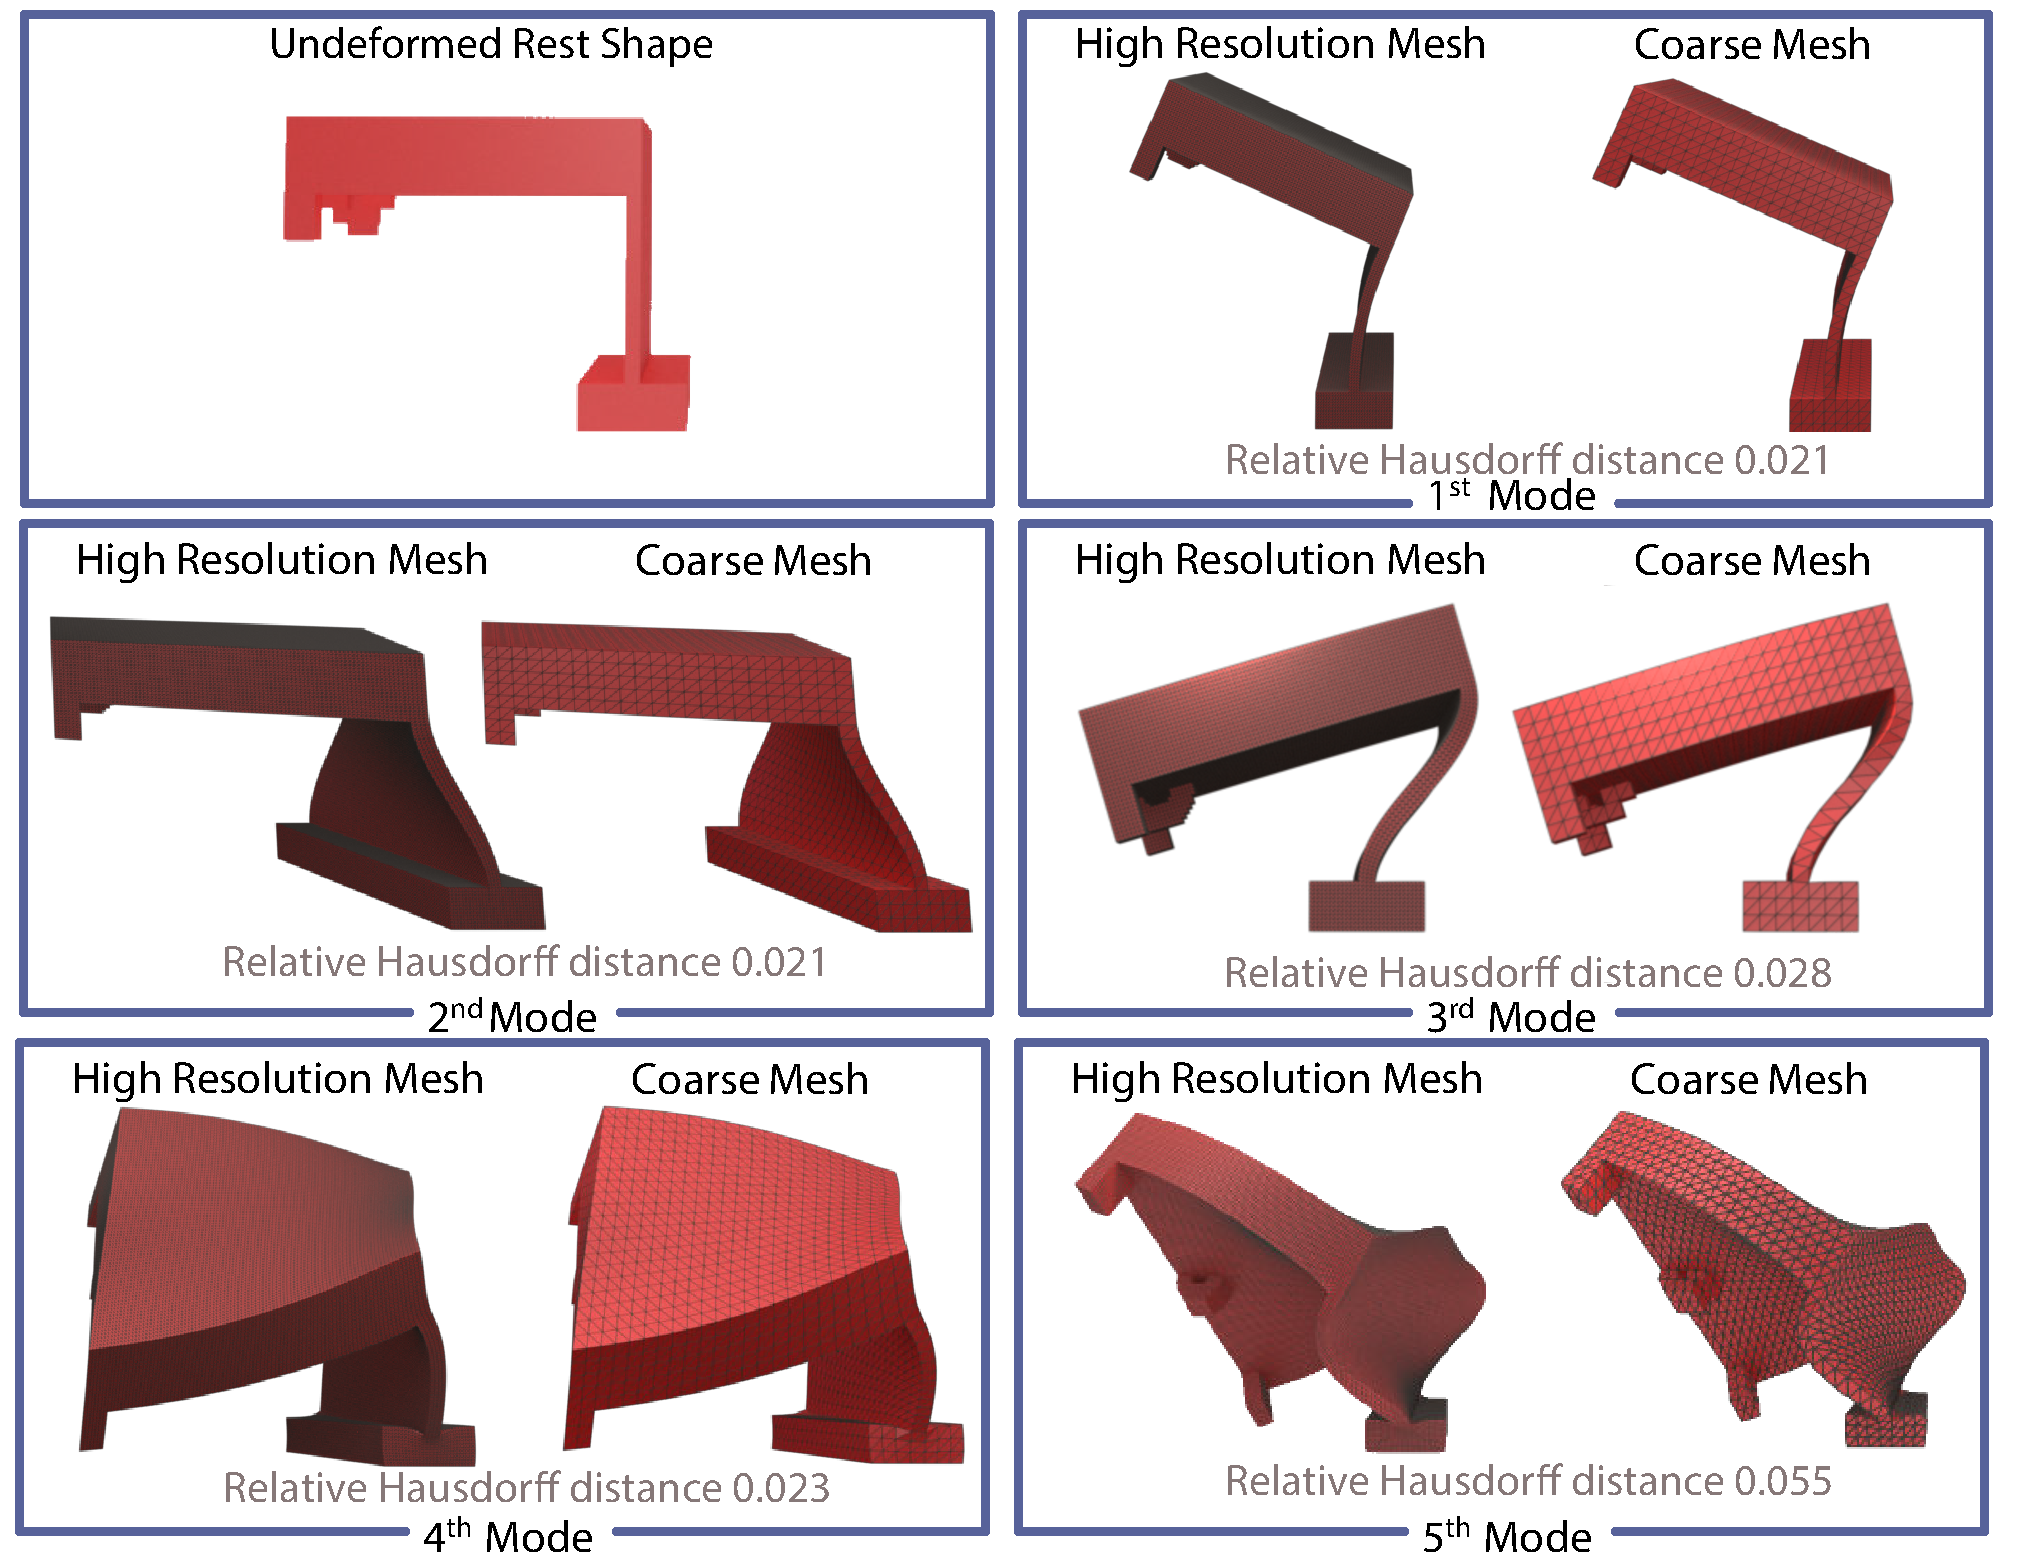
\includegraphics[width=0.5\columnwidth]{images/modeFit3.pdf}
	\caption{Dynamics-aware coarsening (DAC) coarsens meshes to capture deformation with calibrated stiffness. We observe that modal shapes can be replicated up to a quite coarse resolution.}
	\label{fig:defo_and_frequency_match}
\end{figure}

Our geometric coarsening ensures that our DAC mesh captures significant deformation modes of our design accurately.
However, when simulated, these same coarse meshes suffer from numerical stiffening -- an increase in effective stiffness and damping as a consequence of decreased mesh resolution; see Figure~\ref{fig:numerical_stiffness}.
This leads to unacceptably inaccurate simulated trajectories no matter how we simulate this system.
Regaining predictive stiffness and damping by refining the discretization would take us back to intractable mesh sizes.
Rather than refining, we keep our coarse mesh as we have already ensured that our geometry is resolved there and calibrate its frequency spectrum to directly match experiment.
To do this, we rescale our coarse model stiffness so that its fundamental frequency matches an observed frequency. This simple analysis sufficiently recovers effective stiffness and damping to regain a predictive 
nonlinear simulation with our coarse mesh.
\begin{figure}[h]
	\centering
	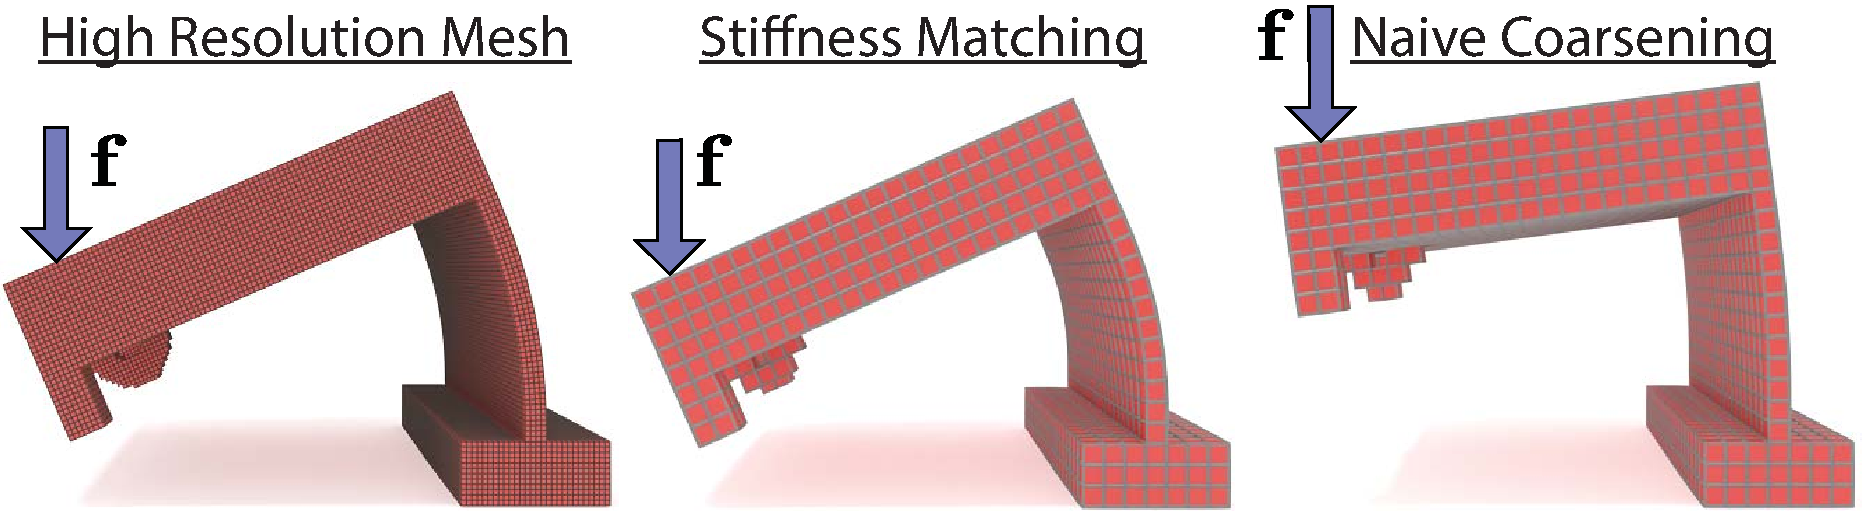
\includegraphics[width=0.5\textwidth]{images/stiffness.pdf}
	\caption{Static Deformation Test. We apply an identical load to three meshes with the same model geometry. With the same material parameters, a high-resolution mesh (left) is effectively 2.5x softer than the corresponding coarse mesh (right). Applying our captured numerical Young's modulus to the coarse mesh (middle) regains the correct deformation of the original, high-resolution mesh on the left.}
	\label{fig:numerical_stiffness}
\end{figure}
\subsection{Boundary Balancing Impact Model}
Traditional momentum-preserving Newmark complementarity integrator has several well-known flaws~\cite{Deuflhard:2008fu}. The Newmark discrete velocity update step in impact response gives rise to an undesirable choice of restitution that is fully elastic (coefficient of restitution $= 1$).
Yet the impact response for elastica along an impact boundary should instead be inelastic with the normal velocity on impact along the elastic boundary dissipated completely~\cite{Doyen:2011gka}.
In turn this results in much too large rebounds upon impact as we observe in preliminary experiments.
A related error for complementarity integrators manifests in commonly observed spurious oscillations in positions and tractions along contact boundaries.
These oscillations are the combined result of instabilities in contact stresses, velocities and displacements.

To address these widely reported problems Deuflhard and colleagues \cite{Deuflhard:2008fu} introduced a contact stabilization step to filter contact response with projection. They observe that contact forces acting on the material boundary should be balanced and so proposed a now-standard FEM contact-stabilization filter (DKE) that applies an L2-projection that zeroes out normal displacements along the boundary of materials at contact interfaces.
This projection on displacement ensures a correct \emph{inelastic} response at the contact boundary and is effective in producing desirably stabilized contact tractions~\cite{Deuflhard:2008fu,Krause:2012im}. 
Nevertheless, when we compare DKE against experiment, we see that the DKE projection likewise introduces unacceptably large rebound errors when compared with real-world results.

To better understand why DKE projection is overly energetic in resolving impacts in our elastic materials, we observe that by projecting out just the normal component of displacement along the boundary,
the DKE method artificially \emph{concentrates} high stresses along the elements just inside the boundary. The concentrated stress effectively load the near-boundary layers which then spring back, introducing a much too large response.
The problem here is that the L2-projection applied is material-oblivious and yet material properties clearly mediate impact response. Compliance distributes contact stresses quickly through an elastic material while, in damped materials, internal friction rapidly attenuates the response. 

With these observations in mind we propose a new Boundary Balancing Impact (BBI) model that can effectively impose boundary force-balance in a material-aware fashion. Starting with our base time integrator we define a compliant, discretization- and material-aware metric for projection. 
This new impact model projects the explicit predicted velocity displacement, to the nearest set satisfying force balance on the boundary with respect to the local approximation of both material \emph{stiffness} and \emph{damping}. The effect of impact is communicated to the material interior while still ensuring that impacts are correctly inelastic along the active contact boundary. 
